\documentclass[12pt,a4paper]{article}
\usepackage[margin=0.8in]{geometry}
\usepackage[T1]{fontenc}\usepackage{lmodern}\usepackage{microtype}\usepackage{graphicx}\usepackage{float}\usepackage{booktabs}\usepackage{longtable}\usepackage{amsmath}\usepackage{hyperref}\usepackage{xurl}\usepackage{enumitem}
\hypersetup{colorlinks=true,linkcolor=blue,urlcolor=blue}\setlength{\parskip}{.4em}\setlength{\parindent}{0pt}
\title{\textbf{GridShift: Short-Horizon Electricity-Demand Forecasting}\\Track B -- Final Research Report}
\author{Abdul Muiz 24L-2501 \textbar{} Abdullah Aftab 24L-2553 \textbar{} Arqum Umais 24L-2591\\AI BDS-5B \textbar{} Instructor: Ms. Bushra Rashid}
\date{November 2026}
\begin{document}\maketitle
\begin{abstract}
This study compares XGBoost, a Long Short-Term Memory network (LSTM), and a Temporal Fusion Transformer (TFT) for next-retained-row electricity-demand forecasting from Indian grid data. After preprocessing, the chronological partitions contain 18,022 training, 3,862 validation, and 3,863 test rows. The target is the next retained observation's demand change, reconstructed to megawatts. On the held-out test set, TFT records the lowest MAE (2,985.18 MW) and RMSE (6,272.79 MW), followed by LSTM (3,567.73; 6,641.47 MW) and XGBoost (4,619.62; 7,930.16 MW). These are reported-run results, not repeated-seed estimates. The LSTM is scored on fewer, later timestamps due to its 168-row sequence window; several timestamp gaps also mean some next-row targets are not exactly one clock-hour ahead. The work supports a cautious ranking on this particular split, not a general claim of superiority or a causal claim about renewable generation.
\end{abstract}
\tableofcontents\newpage
\section{Problem and research question}
Reliable short-horizon demand forecasts inform grid planning. The research question is whether three distinct model families differ in forecast accuracy on a common chronological evaluation of demand, renewable generation, and calendar signals. This is an offline research comparison: no model is connected to live grid operations, and no operational deployment claim is made.
\section{Data, preparation, and task}
The supplied project identifies the data as India's hourly electricity demand, solar, and wind series (Mendeley Data, DOI: \url{https://doi.org/10.17632/y58jknpgs8.2}). The merged input holds 37,392 timestamps; the prepared chronological partitions hold 25,747 rows (70/15/15). The training-only scaler and existing split files are reused. The project README documents 11,714 missing measurement values before interpolation and 11,645 afterward; interpolation is restricted to internal gaps of at most three hours, and rows without usable demand are excluded.

The model target is $\Delta y_t=y_{t+1}-y_t$ and the forecast is $\hat y_{t+1}=y_t+\widehat{\Delta y_t}$. Features include six cyclic calendar encodings, solar and wind, demand lags (1, 2, 24 retained rows), one-row solar/wind lags, and 24- and 168-row rolling demand means. All models use 15 engineered features. There are 4 non-hourly timestamp gaps in validation and 19 in test. Since targets shift by retained row, labels immediately before gaps are not strict one-clock-hour targets; sequences are not reset at those gaps.

\begin{table}[H]\centering\caption{Chronological prepared data and prediction-row counts.}\begin{tabular}{lrrr}\toprule Partition & Prepared rows & XGBoost/TFT predictions & LSTM predictions\\\midrule Train &18,022&17,854&17,687\\ Validation&3,862&3,694&3,527\\ Test&3,863&3,695&3,528\\\bottomrule\end{tabular}\end{table}
\section{Models and evaluation}
\textbf{XGBoost} uses squared-error loss and eight configurations over depth $\{4,6\}$, learning rate $\{0.05,0.10\}$, and 200/400 trees; row and column subsampling are 0.8. Validation MAE selected depth 6, learning rate 0.05, and 200 trees. \textbf{LSTM} uses a 168-row lookback, one layer with 64 units, a linear head, Adam (0.001), batch size 128, and gradient clipping at 1.0. Three settings were compared; the selected run stopped after 16 epochs with its best validation MAE at epoch 11. \textbf{TFT} uses a 168-row encoder; the selected setting has hidden size 48, four attention heads, hidden continuous size 24, dropout 0.15, learning rate 0.002, batch size 64, MAE loss, and Adam. Four configurations were tested.

Validation MAE selected settings; the test partition is held out for final reporting. MAE and RMSE are reported in MW. RMSE weights large errors more heavily. MAPE is retained only where the saved XGBoost metrics report it. No classification metrics are appropriate for this continuous target.
\section{Results}
\begin{table}[H]\centering\caption{Saved validation and test results (MW; lower is better).}\begin{tabular}{llrrl}\toprule Model&Partition&MAE&RMSE&Prediction rows\\\midrule
TFT&Validation&1,566.80&3,316.47&3,694\\ TFT&Test&2,985.18&6,272.79&3,695\\
LSTM&Validation&1,998.05&3,762.90&3,527\\ LSTM&Test&3,567.73&6,641.47&3,528\\
XGBoost&Validation&3,604.19&6,188.10&3,694\\ XGBoost&Test&4,619.62&7,930.16&3,695\\\bottomrule\end{tabular}\end{table}
On this test period, TFT's MAE is about 16% lower than LSTM's and 35% lower than XGBoost's; interpretation is limited by the LSTM timestamp mismatch. Every model has higher test than validation MAE: approximately 90.5% for TFT, 78.6% for LSTM, and 28.2% for XGBoost. This is evidence of a harder later holdout, but a single split does not identify the cause or establish a general distribution-shift mechanism.
\begin{figure}[H]\centering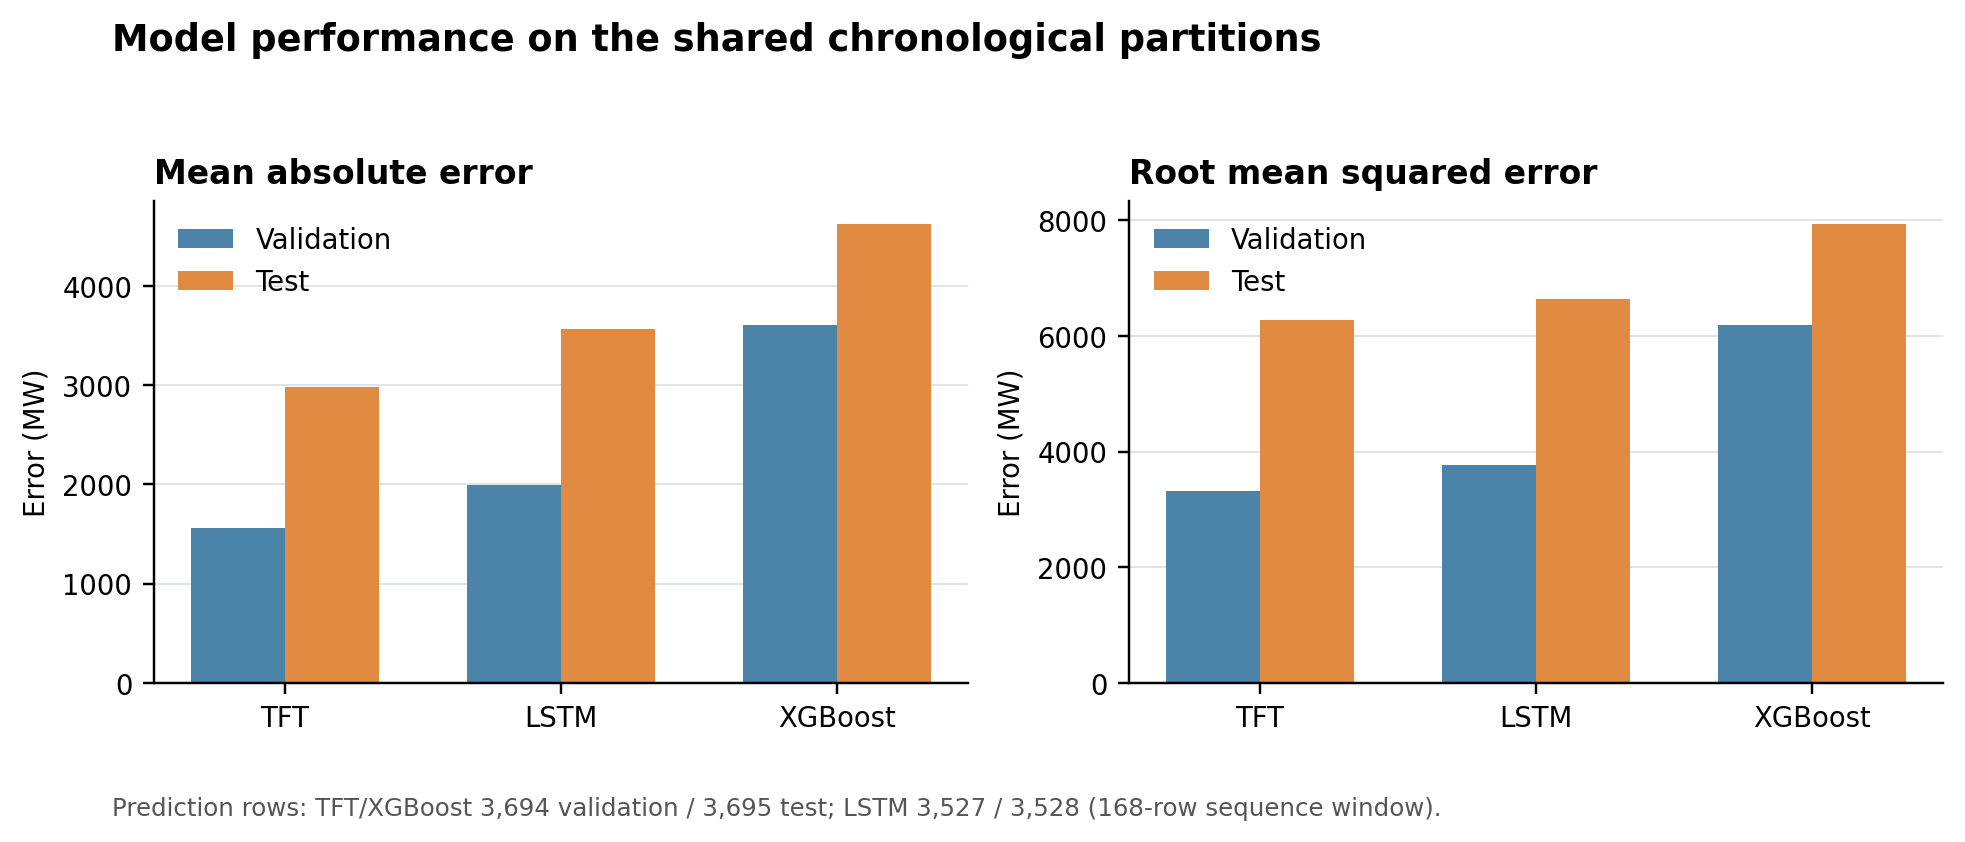
\includegraphics[width=.95\linewidth]{figures/phase5_model_metrics.png}\caption{Validation/test MAE and RMSE. LSTM uses fewer prediction timestamps.}\end{figure}
\begin{figure}[H]\centering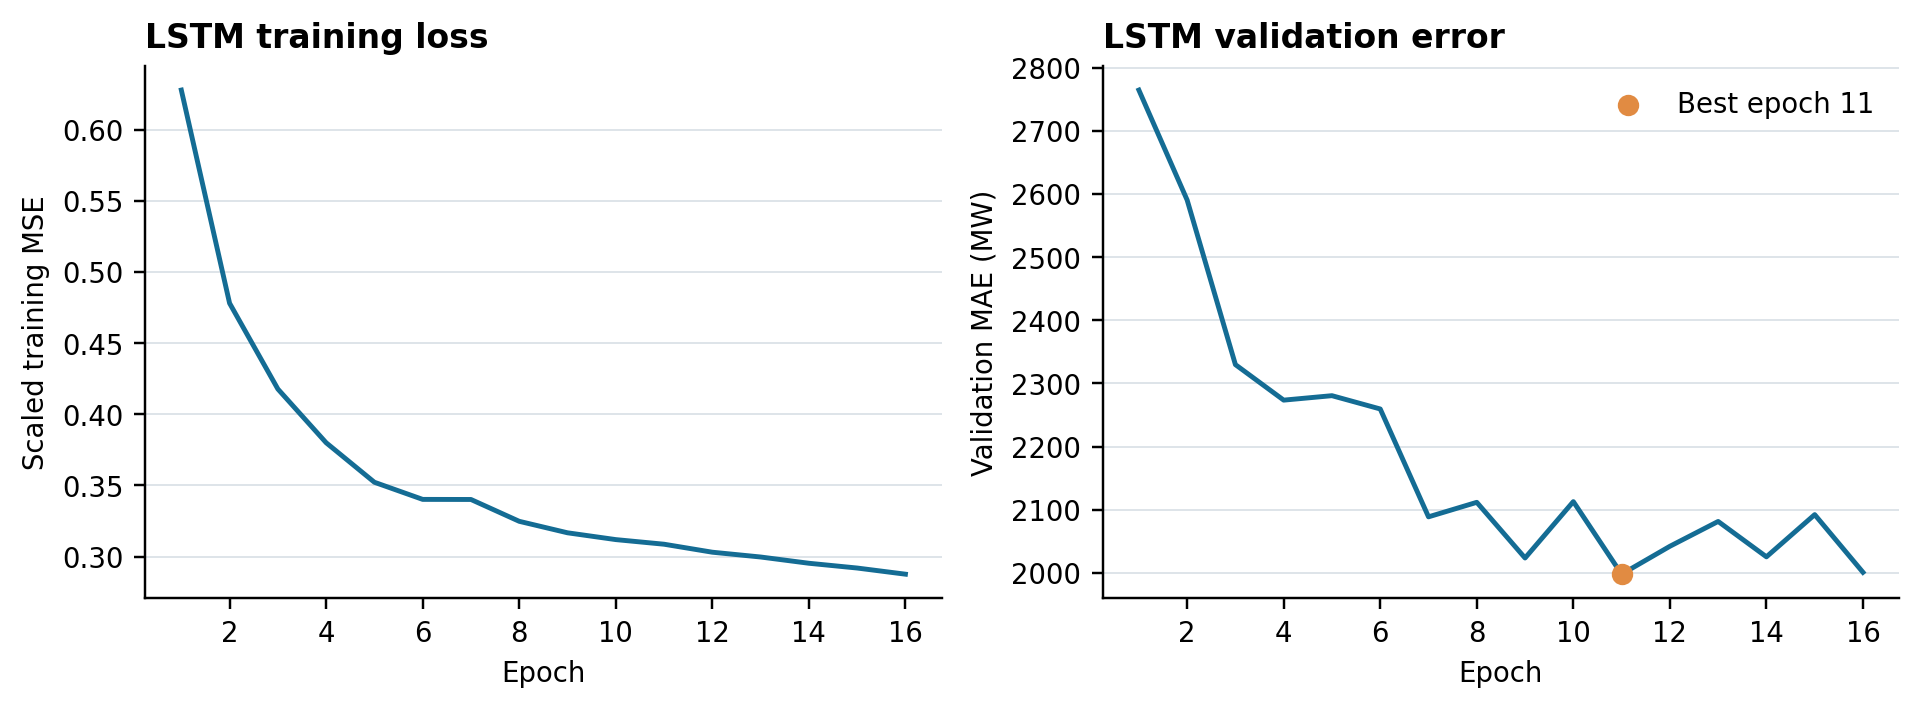
\includegraphics[width=.95\linewidth]{figures/phase5_lstm_history.png}\caption{LSTM training MSE (scaled target) and validation MAE (MW), shown on separate axes.}\end{figure}
\begin{figure}[H]\centering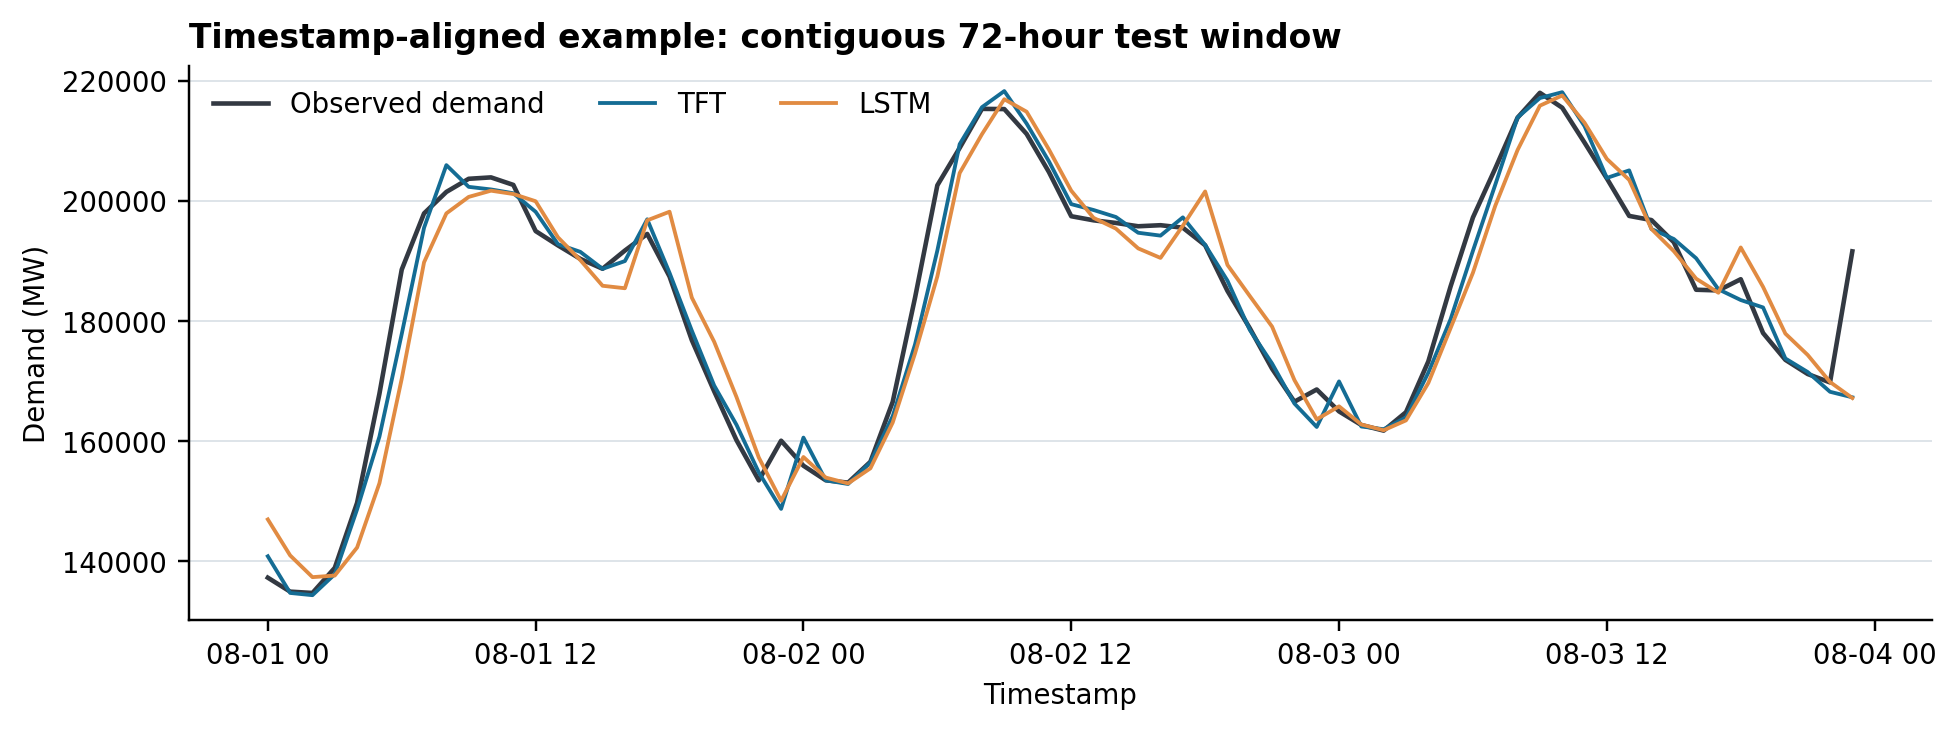
\includegraphics[width=.95\linewidth]{figures/phase5_test_forecasts.png}\caption{Timestamp-aligned contiguous test-period forecast illustration for TFT and LSTM; not a full-period summary.}\end{figure}
\section{Ablation and component contribution}
The supplied results contain hyperparameter searches but no controlled component-removal experiment. Consequently, this report does not attribute the observed ranking to attention, recurrence, feature selection, lookback length, or renewable inputs. Hyperparameter comparisons are not architecture ablations. The following ablation plan is the next experimental step; values must be measured on the same splits and timestamp intersection before drawing component-level conclusions:
\begin{enumerate}[leftmargin=*]
\item \textbf{Input groups:} full feature set versus removing solar/wind features; versus removing calendar encodings; versus removing lag/rolling features.
\item \textbf{Temporal context:} compare 24-, 72-, and 168-row lookbacks, keeping optimization budget and selection rule fixed.
\item \textbf{TFT structure:} compare full TFT with attention disabled or reduced, and variable-selection components removed where supported by the implementation; document any implementation changes.
\item \textbf{LSTM capacity:} compare one versus two layers and 32 versus 64 units while holding data, early stopping, and seeds fixed.
\item \textbf{Controls:} add persistence ($\hat y_{t+1}=y_t$) and seasonal-naive ($\hat y_{t+1}=y_{t-24}$ when truly hourly) baselines. Report identical timestamps and multiple random seeds for neural models.
\end{enumerate}
\section{Error analysis, interpretation, and limitations}
The saved LSTM test analysis reports underprediction on average (mean signed error $-208.54$ MW) and larger errors in the lowest-demand quartile (MAE 4,365 MW); it tends to overpredict that lowest quartile and underpredict the highest. Hour 23 is difficult for both recurrent and transformer predictions: LSTM test MAE is reported as 12,063 MW and TFT test MAE as 12,640 MW. These are targeted summaries, not explanations of individual failures. Plausible mechanisms such as ramping, abrupt demand changes, or temporal gaps require sample-level diagnostics before they can be asserted.

Key limitations are: (i) one chronological holdout and no uncertainty intervals or repeated-seed estimates; (ii) model metrics are not fully timestamp-matched because LSTM requires a sequence; (iii) retained-row target construction makes some labels non-hourly; (iv) gaps are not used to reset sequence windows; (v) no persistence/seasonal-naive baseline in the reported comparison; (vi) component ablations have not been run; (vii) no external weather or region-level covariates are established in the supplied inputs; and (viii) results depend on the supplied prepared files and have not been independently rerun here. Renewable-demand correlation is not evidence that renewable generation caused demand changes.
\section{Reproducibility and viva demonstration}
The supplied repository includes model scripts, prepared split CSVs, metrics, predictions, settings, and checkpoints. Run the data/model pipeline from the project root using the repository's documented dependencies and commands; preserve the existing split manifest and avoid regenerating splits when comparing with these saved results. For viva, demonstrate the experimental codebase: show the shared split loader, forecast target construction, saved prediction outputs, and metric-generation workflow. The current Track B evidence supports demonstrating reproducible offline experiments; it does not claim a hosted inference application.
\section{Conclusion}
Among the three saved runs, TFT has the lowest reported error on validation and test, with LSTM second and XGBoost third. The ranking is promising for the TFT configuration on this dataset and split, but not yet a robust model-selection conclusion because of timestamp alignment, the later-period error increase, and the absence of ablation, naive baselines, and repeated seeds. These caveats should be resolved before translating the result into operational or broad generalization claims.

\newpage
\section{Introduction and motivation}
Electricity-demand forecasting is a decision-support problem: the forecast is useful only insofar as its horizon, information set, error profile, and operational context match the decision being supported. Short-term load prediction has long been approached with statistical, machine-learning, and neural methods. Prior TFT work has applied the architecture to short-term city load and compared it with statistical and recurrent alternatives, illustrating the relevance of benchmarking rather than assuming an architecture is universally best \cite{pham2022}. The present project narrows the question to a single prepared Indian grid-level series and one-step forecasting, and therefore treats all model conclusions as specific to this dataset, split, and feature set.

A recurring risk in machine-learning comparisons is that design choices--particularly the split, information available at prediction time, preprocessing, tuning, and evaluation sample--can dominate apparent model differences. Time-series observations are ordered and dependent. Random shuffling can allow future observations to influence training or validation and does not reproduce forecasting deployment. A final chronological holdout is a defensible first estimate, while blocked or rolling-origin evaluation can use multiple historical forecast origins and support more robust selection \cite{bergmeir2012}. Accordingly, this study treats the supplied final holdout as a limited experiment and identifies rolling-origin evaluation as a priority extension.

\subsection{Research objectives}
The work has five objectives: define a reproducible next-step demand-change prediction task; compare tree-based, recurrent, and transformer-based methods under chronological partitions; report interpretable error metrics in physical units; inspect time-of-day and demand-level error patterns where saved prediction outputs permit; and identify the additional experiments required before architecture-level conclusions can be made.

\subsection{Research questions}
\begin{enumerate}[leftmargin=*]
\item What are the validation and test MAE and RMSE of the three supplied model runs on the prepared partitions?
\item Does the ranking observed on the test partition agree with the validation-based model-selection ranking?
\item Which caveats in timestamp coverage, sample alignment, feature construction, and experimental design materially constrain that comparison?
\item What controlled experiments are necessary to attribute performance differences to model components rather than to model-family or configuration differences?
\end{enumerate}

\subsection{Scope and non-claims}
The analysis concerns the saved offline forecast experiment, not deployment. It does not estimate the causal effect of solar or wind generation on demand; does not provide uncertainty-calibrated intervals; does not claim that TFT is state of the art across grids or horizons; and does not establish that forecast errors would be acceptable for dispatch, reserve scheduling, or market participation. No inference about regional subgrids, households, or demographic equity is possible from this aggregate series.

\newpage
\section{Related work and conceptual framing}
Short-term electricity-demand forecasting spans conventional time-series methods, supervised tree ensembles, recurrent neural networks, and attention-based architectures. The methods represent different inductive biases: trees partition engineered feature space, recurrent networks compress sequential histories, and TFT combines recurrent processing with attention and variable-selection mechanisms. A direct empirical comparison is informative only when the compared systems see the same forecast-available inputs and when the evaluation windows are comparable.

TFT has been applied to electricity load forecasting with historical load, weather, and calendar variables, and has been compared with statistical and recurrent baselines in a city-level setting \cite{pham2022}. That work motivates inclusion of TFT as a candidate, not an expectation that it must win here. The selected GridShift configuration is a one-step adaptation with a 168-row encoder, rather than a claim to reproduce every original TFT use case. The differences in population, features, target, horizon, preprocessing, and training implementation preclude treating another paper's performance as directly comparable.

The broader methodological literature emphasizes that time-series predictor evaluation differs from exchangeable-data cross-validation. Bergmeir and Benítez describe the use of a final segment for testing and discuss blocked cross-validation as an option for evaluating time-series predictors under suitable assumptions \cite{bergmeir2012}. GridShift's single chronological split respects ordering, but it gives only one estimate of future-period performance. A sequence of forecast origins would reveal whether the ranking is stable across periods and whether the observed deterioration is specific to the selected test interval.

\subsection{Why include multiple model families?}
XGBoost is a strong tabular comparator when lags and rolling statistics make temporal structure explicit. LSTM provides a recurrent sequence-learning comparator in which the temporal window is consumed directly. TFT supplies an architecture with learned feature selection and attention components. Their comparison is useful as a systems benchmark, but it cannot isolate the causal contribution of attention, recurrence, or feature selection because the model families also differ in optimization, losses, effective sample count, and parameterization.

\subsection{Benchmarking principle}
A model's error should be judged against a meaningful baseline and across repeated forecast origins. In this project, the saved metrics compare three learned models but do not include persistence or seasonal-naive predictions. Prior short-term load research also compares TFT with statistical and recurrent alternatives, underscoring the value of explicit baselines rather than architectural assumptions \cite{pham2022}. Thus the results establish a relative ordering among these saved runs only; they do not establish that any model improves on a minimally complex operational benchmark. This distinction is central to interpreting the project's comparative claim.

\newpage
\section{Data provenance and data-quality audit}
The supplied project documentation cites the Mendeley Data record for hourly Indian electricity demand, solar generation, and wind generation \cite{dataset}. The project's merged input has 37,392 timestamped rows, while the cleaned split files retain 25,747. The archived project identifies a discrepancy between coverage described in the data record and the period apparent in the merged file; metadata and timestamp coverage should therefore be reconciled against the original workbook and source record before publication. This report does not silently resolve that provenance discrepancy.

\subsection{Audit trail and cleaning sequence}
The project describes a process that removes empty records, parses timestamps, converts measurements to numeric values, performs limited interpolation over short internal gaps, retains outlier flags rather than deleting extreme observations, derives cyclic calendar features, creates chronological partitions, and fits a scaler on training data only. The reported missing-measurement count falls from 11,714 to 11,645 after interpolation. These counts are drawn from the supplied cleaning report and should be accompanied in a formal release by the exact input workbook checksums and audit JSON.

\begin{longtable}{p{.23\linewidth}p{.69\linewidth}}
\caption{Data-processing operations and the associated reproducibility question.}\\
\toprule Operation & Audit question for a reproducible release \\\midrule\endfirsthead
\toprule Operation & Audit question for a reproducible release \\\midrule\endhead
Timestamp parsing & What timezone, daylight-saving convention, and source-specific timestamp format were used? Were timestamps unique after merge?\\
Resampling and gaps & Which timestamps were expected, which were absent, and how were daylight-saving or source publication gaps distinguished?\\
Interpolation & Were only internal gaps of at most three hours interpolated? Were interpolated values logged separately from observed values?\\
Target availability & Were rows with missing load removed only after interpolation? What is the retained timestamp list for each split?\\
Outlier handling & Were flagged values retained? Were thresholds calculated on training data or across all observations?\\
Scaling & Were scaler parameters fitted on the training subset and serialized for reuse?\\
Split boundaries & What are the exact inclusive start and end timestamps of train, validation, and test?\\
\bottomrule\end{longtable}

The key reproducibility weakness is not the absence of all processing documentation: the archive contains an audit report and prepared split files. Rather, the manuscript needs the exact split dates, data file provenance, preprocessing code version, and enough metadata to regenerate each row deterministically. The follow-up release should include a manifest with source filename, checksum, timestamp range, row counts at each processing stage, split boundaries, scaler parameters, and software versions.

\subsection{Missingness and interpolation}
Short-gap interpolation can preserve continuity for models that expect sequential inputs, but it also replaces observed data with estimates. Missingness may be systematic; for example, a long outage or a particular source reporting pattern could align with distinctive operating conditions. Therefore, the number and timing of imputed values should be summarized by variable and by partition. A sensitivity run that excludes imputed target rows, and another that carries explicit missingness indicators, would establish whether the current imputation policy materially affects results.

\subsection{Outliers and extreme demand}
Keeping IQR-flagged observations rather than deleting them is a defensible choice because high loads can be genuine. However, the threshold definition, flag counts, and model-specific influence of extreme periods should be documented. MAE is relatively interpretable as a typical absolute miss, whereas RMSE gives disproportionate weight to large errors. The gap between MAE and RMSE in all reported models indicates that large residuals contribute materially to squared error, but the saved summary alone does not identify which operational events produced them.

\newpage
\section{Forecasting task and information set}
The supplied implementation forecasts the change between a current retained row and the next retained row. At forecast origin $t$, the target is $\Delta y_t=y_{t+1}-y_t$, and the reconstructed level forecast is $\hat y_{t+1}=y_t+\widehat{\Delta y_t}$. Under a complete regular hourly series this would correspond to a one-hour-ahead task. Because the retained sequence contains non-hourly gaps, the strictly accurate wording is next-retained-row prediction, with nominal one-hour intent.

\subsection{Feature dictionary}
\begin{longtable}{p{.22\linewidth}p{.32\linewidth}p{.37\linewidth}}
\caption{Shared engineered input features described by the project.}\\
\toprule Feature family & Columns or construction & Interpretation and caution \\\midrule\endfirsthead
\toprule Feature family & Columns or construction & Interpretation and caution \\\midrule\endhead
Calendar cycle & hour, weekday, month sine/cosine & Encodes cyclical position; verify timezone and calendar basis.\\
Renewables & Current solar and wind generation & Use only values available at the forecast origin; contemporaneous measurements may not be operationally available without latency assumptions.\\
Load lags & $y_{t-1}, y_{t-2}, y_{t-24}$ by retained row & Across gaps, row lags do not always equal elapsed-hour lags.\\
Renewable lags & Solar and wind at prior retained row & Same retained-row caveat applies.\\
Rolling means & Load averages over 24 and 168 retained rows & Summaries can span elapsed times longer than the nominal window when missing rows exist.\\
\bottomrule\end{longtable}

The information-set audit should ask not only whether a feature is numerically present, but whether it would be known at the intended decision time. Calendar features are known in advance. Demand and renewable measurements are historical observations subject to publication and telemetry delays. A deployment-oriented study would define data latency, revision policy, and forecast issuance time, then construct features from the exact information set available at that time.

\subsection{Gap boundary consequences}
The archived project notes four non-hourly intervals in validation and 19 in test. The target uses the next retained row and feature sequences are not reset at gaps. Therefore, a target just before a gap may be several hours ahead, while lag features continue to be indexed by retained-row order. Such samples are not strictly comparable to complete-hour samples. The primary reanalysis should either restore a complete hourly index and handle missing values explicitly, or exclude forecast origins whose target interval is not exactly one hour, reporting both the original and strict-hour results.

\newpage
\section{Model implementations}
\subsection{XGBoost}
The XGBoost model uses a squared-error objective over the common engineered features, following the gradient-boosted tree framework introduced by Chen and Guestrin \cite{xgboost}. Eight hyperparameter combinations vary maximum depth (4 or 6), learning rate (0.05 or 0.10), and estimator count (200 or 400); row and column subsampling are each fixed at 0.8. The selected setting is depth 6, learning rate 0.05, and 200 estimators based on validation MAE. The implementation is a tabular learner: sequence structure enters through explicit lag and rolling features rather than through a recurrent state.

\subsection{LSTM}
The LSTM receives a 168-row by 15-feature lookback sequence and follows the recurrent memory-cell family introduced by Hochreiter and Schmidhuber \cite{lstm}. and maps the final representation through a linear head to a demand-change prediction. The selected configuration has one recurrent layer with 64 hidden units and no dropout. Training uses Adam with learning rate 0.001, batch size 128, MSE on the training-scaled target, gradient clipping at 1.0, and validation MAE for selection and early stopping. The selected run's minimum validation MAE occurs at epoch 11; training ends at epoch 16 under the documented stopping rule. The training objective and selection metric differ in form and scale, so their numerical values must not be compared directly.

\subsection{Temporal Fusion Transformer}
The TFT implementation uses a 168-row encoder and draws on the temporal fusion architecture described by Lim et al. \cite{tft}. and one-record horizon, with hidden size 48, four attention heads, hidden continuous size 24, dropout 0.15, learning rate 0.002, and batch size 64. The selected run minimizes MAE and uses Adam with gradient clipping. Four configurations were tested and validation MAE selects the larger configuration. This is the best of the tested settings, not evidence that these hyperparameters are globally optimal.

\subsection{Architecture and parameter reporting}
For a journal-ready submission, the implementation report should include the exact library versions and model-construction arguments, parameter counts, random seeds, deterministic settings, hardware, checkpoint-selection rule, and the code commit identifier. The archive contains model scripts, selected-setting JSON files, metrics, predictions, and checkpoints, but a results paper should make these supporting materials accessible alongside the manuscript. The current report does not infer undocumented parameter counts or runtime.

\newpage
\section{Experimental protocol}
\subsection{Chronological partitioning}
The project uses chronological 70/15/15 train, validation, and test partitions with 18,022, 3,862, and 3,863 prepared rows. Validation selects configurations; test estimates final held-out performance. The scaler is fit on training only. The primary quality-control requirement for future re-runs is to freeze and report exact boundary timestamps and prevent test data from influencing feature selection, hyperparameter choice, or stopping.

\subsection{Model selection and tuning budget}
The candidate configurations differ by family: XGBoost tests eight combinations, LSTM three settings, and TFT four. Such searches do not have equal effective capacity or equal compute. The selected models therefore constitute a practical comparison of the supplied tuning procedures, not a compute-matched tournament. A stronger study would predefine a tuning budget per model, use the same validation protocol, log every trial, and ensure that test data are opened only once after selection.

\subsection{Evaluation sample alignment}
XGBoost and TFT produce 3,694 validation and 3,695 test predictions. LSTM produces 3,527 and 3,528 because its sequence window omits early rows from each partition. Thus the reported model metrics are not calculated over precisely identical timestamps. This could change a ranking if the omitted timestamps are unusually easy or difficult. The fair comparison should join predictions by timestamp and compute all three models' metrics over the intersection, then separately report each model's full available-window performance.

\subsection{Forecast origins and future protocol}
A robust extension should use expanding-window or rolling-origin evaluation with several chronological cut points. Every fold should include a training interval, a validation interval for selection, and an untouched evaluation interval. The origin list, window length, retraining frequency, and horizon must be specified before running. This would support reporting mean and dispersion of performance across origins and reveal whether model rankings vary across seasons or demand regimes. Time-series evaluation literature supports careful temporal validation and cautions against treating ordinary random cross-validation as interchangeable with forecasting evaluation \cite{bergmeir2012}.

\newpage
\section{Metrics and statistical interpretation}
For errors $e_i=\hat y_i-y_i$, the project reports mean absolute error and root mean squared error:
\[
\mathrm{MAE}=\frac{1}{n}\sum_{i=1}^{n}|e_i|,\qquad
\mathrm{RMSE}=\sqrt{\frac{1}{n}\sum_{i=1}^{n}e_i^2}.
\]
Both are expressed in MW. MAE answers the average absolute miss in the target unit. RMSE increases more strongly with large residuals. Neither metric alone describes calibration, signed bias, peak-specific performance, or economic consequences. XGBoost's saved output additionally reports MAPE; the report does not create MAPE for the other models because it was not in their supplied metric files.

\subsection{Why classification scores are excluded}
The target is continuous demand change reconstructed to continuous demand. Precision, recall, F1, and ROC-AUC would require a threshold-defined event label such as peak/non-peak or ramp/no-ramp. No such decision threshold is specified, so these classification metrics would not answer the current research question.

\subsection{Uncertainty and paired comparison}
The saved summaries provide point estimates only. Because forecasts are evaluated on temporally ordered, autocorrelated data, naive independent-sample standard errors would not be justified without additional assumptions. A follow-up can compare timestamp-paired absolute errors over identical windows and use block-based resampling over time or multiple rolling origins to quantify variability. Any inferential test should be specified before examining the result and should preserve temporal dependence. No confidence interval or significance claim is made in this report.

\subsection{Operational interpretation}
An error measured in MW is not automatically operationally meaningful or acceptable. Utility use would require a stated decision, an acceptable error tolerance, a comparison with current practice, evaluation during peaks and ramps, uncertainty characterization, monitoring for drift, and a safe fallback. This project does not supply those elements and should remain an academic forecasting prototype.

\newpage
\section{Detailed comparative results}
The saved metrics consistently rank TFT first, LSTM second, and XGBoost third on both validation and test MAE and RMSE. The gap between the models is material in absolute terms but should be interpreted within the non-identical evaluation timestamp caveat for LSTM. In the held-out test metrics, TFT's MAE is about 16.3\% lower than LSTM's and 35.4\% lower than XGBoost's, calculated relative to the comparator MAE. These are descriptive comparisons of saved point estimates, not uncertainty-adjusted effects.

\begin{table}[H]\centering\caption{Derived test-period differences relative to each comparator.}\begin{tabular}{lrr}\toprule Comparison & MAE difference (MW) & Relative reduction vs comparator \\\midrule TFT vs LSTM & 582.55 & 16.3\%\\ TFT vs XGBoost & 1,634.44 & 35.4\%\\ LSTM vs XGBoost & 1,051.89 & 22.8\%\\\bottomrule\end{tabular}\end{table}

Each model's test error is higher than its validation error. Relative MAE increases are approximately 90.5\% for TFT, 78.6\% for LSTM, and 28.2\% for XGBoost. The differing magnitudes suggest that model performance changed across the two periods, but the report cannot attribute the increase to concept drift, seasonality, missingness, events, or model overfit without additional diagnostic analyses. A single validation/test boundary does not separate those explanations.

\subsection{Reading MAE and RMSE together}
RMSE exceeds MAE by a substantial margin for every model. That pattern is consistent with a residual distribution containing some large misses, though it does not alone identify their count or cause. A professional error report should complement aggregate metrics with residual quantiles, signed bias, peak-load subsets, ramp subsets defined in advance, and error by hour and month. Subgroup metrics should report the number of observations in each cell so small groups are not overinterpreted.

\subsection{XGBoost MAPE}
The XGBoost CSV reports validation MAPE of 1.93\% and test MAPE of 2.42\%. MAPE is scale-relative and can behave poorly when actual values approach zero; the demand series here is high and positive, but comparability remains limited because other models' MAPE is not present in their metric files. MAE and RMSE remain the primary cross-model metrics in this manuscript.

\newpage
\section{Error analysis and failure modes}
The archived project reports that LSTM test predictions have mean signed error of $-208.54$ MW, corresponding to modest average underprediction under the convention prediction minus actual. It also reports a highest test MAE of 4,365 MW in the lowest actual-demand quartile, with a tendency to overpredict the lowest quartile and underpredict the highest. For hour 23, reported test MAE is 12,063 MW for LSTM and 12,640 MW for TFT. These observations identify candidate error modes, but they do not explain why the errors occurred.

\subsection{Interpretive hypotheses requiring tests}
Several mechanisms could plausibly contribute to high errors at certain hours: changes in evening demand ramps, unusual renewable output, missing or imputed measurements, irregular timestamp intervals, or distribution changes between validation and test. These are hypotheses, not conclusions. Testing them requires joining residuals to timestamps and predictors, defining ramp/peak strata before analysis, and comparing the findings across forecast origins. Sample-level error narratives should be supported by raw data checks and not selected only because they fit a preferred story.

\subsection{Recommended residual diagnostics}
A complete analysis should include residuals over time, a histogram or density plot, quantiles of absolute and signed error, error versus actual demand, error by hour and month, peak and ramp subsets, and a list of the largest errors with timestamp, actual, forecast, recent history, and gap/imputation flags. For every plot, show the number of observations and indicate if axes or filters change across models. If the residual series exhibits autocorrelation, report it as a diagnostic and consider whether model errors cluster during extended regimes.

\subsection{Failure taxonomy}
For review and viva preparation, error cases can be categorized as: data-quality issue (timestamp or measurement), target interval mismatch, extreme but valid observation, rapid ramp, ordinary variation, or model misspecification. Assigning a category requires inspecting case context; the current aggregate results do not permit a reliable count by category. This taxonomy is a proposed annotation protocol, not a result of the current experiment.

\newpage
\section{Ablation study: status and executable design}
\subsection{What the current evidence does and does not show}
The provided archive contains hyperparameter trials and selected model settings, but no controlled component-removal ablation. It therefore cannot answer which individual architecture component contributed most to performance. A full TFT-versus-LSTM-versus-XGBoost comparison is not an ablation: architecture, objective, sequence handling, tuning search, and optimization all change together. This distinction is necessary for scientific attribution.

\subsection{Pre-registered ablation matrix}
\begin{longtable}{p{.16\linewidth}p{.31\linewidth}p{.28\linewidth}p{.17\linewidth}}
\caption{Recommended controlled ablation matrix. Each variant must be trained and evaluated under the same split and seeds.}\\
\toprule Family & Full model & Removal or alternative & Primary comparison \\\midrule\endfirsthead
\toprule Family & Full model & Removal or alternative & Primary comparison \\\midrule\endhead
Features & All 15 common inputs & Remove renewable variables & Does renewables' information add predictive value?\\
Features & All 15 common inputs & Remove calendar cyclic terms & Does calendar context add value beyond lags?\\
Features & All 15 common inputs & Remove lag/rolling features & How much comes from engineered autoregressive inputs?\\
Lookback & 168-row context & 24 and 72 rows & Does longer context improve held-out performance?\\
LSTM & 64-unit, one-layer & 32-unit; two-layer; no sequence controls & Is capacity associated with stable gains?\\
TFT & Selected full architecture & Disable/alter attention or variable selection where supported & Which TFT mechanism contributes?\\
Target treatment & Difference prediction & Direct level prediction & Does differencing aid optimization or accuracy?\\
Missingness & Current imputation policy & Complete-hour-only sample; missingness flags & Are results sensitive to gap handling?\\
\bottomrule\end{longtable}

\subsection{Controls and interpretation}
For every ablation, freeze split boundaries, seed, tuning budget, stopping rule, features not under test, and prediction timestamp set. Report mean and standard deviation across at least several predeclared seeds for neural models, plus a paired per-timestamp error comparison. Do not infer a component's causal contribution from one run if the change also alters capacity or training budget. If a library implementation cannot remove a component cleanly, describe the substitute model and the resulting construct-validity limitation.

\subsection{Simple baselines}
Add persistence, where the next demand is forecast as current demand, and a seasonal-naive baseline using the previous same-hour value only when the series has a true 24-hour interval. These baselines establish whether the learned systems add value beyond simple temporal persistence. The existing 24-row lag is based on retained rows and may not represent exactly 24 elapsed hours across gaps; baseline construction should use timestamps rather than row positions.

\newpage
\section{Threats to validity}
\subsection{Construct validity}
The operational objective is phrased as hourly demand forecasting, while the implemented target is next retained-row forecasting. Non-hourly gaps therefore create a mismatch between the construct and some target intervals. The project should distinguish nominal horizon from verified elapsed-time horizon and report a strict one-hour subset.

\subsection{Internal validity}
Different models use different training losses and sequence mechanisms, and the tuning budgets differ. LSTM has fewer evaluation timestamps. There is no controlled ablation, randomized seed replication, or paired statistical uncertainty. These factors prevent a strong attribution of observed differences to architecture alone.

\subsection{External validity}
One aggregated Indian series and one chronological holdout cannot establish performance on other grids, seasons, regions, demand scales, or operational systems. Findings should not be transferred to distribution-level loads or other countries without external validation. The dataset's provenance/date discrepancy also warrants reconciliation before a publication-quality claim about coverage.

\subsection{Conclusion validity}
Point estimates can change under alternate holdout boundaries and sample alignment. No interval estimates or multiple-origin results are supplied. A rank ordering on one holdout is suggestive, but not a stable estimate of comparative performance. Claims of statistically significant superiority are not warranted.

\subsection{Selection and reporting bias}
Configurations were selected by validation MAE and then reported on test. That is appropriate in principle, provided test results were not used in iterative model changes. The audit trail should document when test predictions were first inspected, all attempted trials, and any changes made after that inspection. If results were iteratively refined using test feedback, a new untouched period is needed for a confirmatory estimate.

\newpage
\section{Reproducibility, artifacts, and reporting checklist}
The supplied project supports partial reproducibility through model scripts, prepared CSV files, settings JSON, metrics, predictions, and checkpoints. A complete archival package should also include a lockfile or exact dependency versions, operating system and hardware description, random seeds, full training logs, source data checksum, split manifest with timestamps, scaler artifact, and the exact commit for the run. Model checkpoints alone are insufficient to reproduce training or explain model selection.

\begin{longtable}{p{.06\linewidth}p{.65\linewidth}p{.21\linewidth}}
\caption{Pre-submission reproducibility checklist.}\\
\toprule Done? & Item & Status in supplied evidence \\\midrule\endfirsthead
\toprule Done? & Item & Status in supplied evidence \\\midrule\endhead
$\circ$ & Exact data citation, version, license, original filenames, and checksums & Partial: DOI cited; checksum not in report\\
$\circ$ & Data audit with schema, units, timestamps, and exclusions & Partial: audit artifacts present\\
$\circ$ & Exact train/validation/test timestamp boundaries & Needs inclusion\\
$\circ$ & Forecast horizon and information set defined by timestamp & Partial: gap mismatch disclosed\\
$\circ$ & Preprocessing and missing-data policy documented & Described; validate full pipeline reproduction\\
$\circ$ & Feature availability and leakage review & Needs explicit row-level audit\\
$\circ$ & Seeds, software versions, device, and deterministic settings & Needs inclusion\\
$\circ$ & All trials and model-selection criterion reported & Search summaries included; full logs should be retained\\
$\circ$ & Test evaluation kept untouched until selection & Confirm from experiment history\\
$\circ$ & Metrics computed on a common timestamp intersection & Not yet; priority analysis\\
$\circ$ & Baseline models and component ablations & Not present; planned\\
$\circ$ & Residual diagnostics and uncertainty across origins & Partial diagnostic summary; no uncertainty\\
$\circ$ & Code, configuration, data manifest, and prediction files archived & Code/results present in supplied project\\
\bottomrule\end{longtable}

\subsection{Viva demonstration plan}
The research-track viva can demonstrate: (1) the data audit and cleaning report; (2) the chronological split and train-only scaler; (3) target/feature construction; (4) one model training script and checkpoint; (5) validation-based selection; (6) saved test predictions and metric computation; and (7) the report's limitations and next experiments. The demonstration should make clear that this is a reproducible offline experiment, not a live forecasting service.

\newpage
\section{Discussion}
The most defensible result is a descriptive one: among the saved, validation-selected runs, TFT records the smallest error on the supplied test partition, LSTM is second, and XGBoost is third. The result is coherent across MAE and RMSE, and TFT also leads on validation. Nevertheless, the comparison is not yet fully fair because LSTM predictions cover fewer timestamps, the exact hourly target is violated immediately before some gaps, and model families have unequal tuning spaces. A timestamp-intersection re-score is the most immediate analytical correction.

The rise in test-period errors for all methods is a warning against relying on validation alone. It may indicate a harder later period, but the present evidence cannot establish whether the cause is distribution shift, a seasonal boundary, outliers, missingness, or a modelling limitation. A rolling-origin evaluation is needed to distinguish a stable degradation pattern from a single-period anomaly. The high reported hour-23 errors and demand-quartile asymmetry offer focused diagnostic leads, but should be checked with counts, aligned timestamps, and repeated periods before they are presented as robust subgroups.

The supplied design has useful strengths: chronological partitions are used; the scaler is fitted on training only; multiple model families are compared; saved predictions and tuning summaries exist; and the report discloses important timestamp limitations. The strongest improvement is not adding more neural architectures, but tightening the evaluation protocol: establish exact elapsed-time targets, align evaluation timestamps, include persistence baselines, and quantify variation across forecast origins and random seeds. These steps make the comparison more scientifically informative than a longer hyperparameter search on the same split.

\subsection{Practical implication}
The current result can guide a follow-up experiment, not a deployment choice. A lower point error on one holdout is insufficient to establish reliability for grid decisions. Deployment would require operationally available inputs, latency and missing-data handling, uncertainty and fallback behavior, peak/ramp evaluation, drift monitoring, and approval against a decision-specific tolerance. No such operational validation is reported here.

\newpage
\section{Conclusion and next decision gate}
The saved experiment ranks TFT first, LSTM second, and XGBoost third by both test MAE and RMSE. This supports selecting TFT as the leading candidate for a carefully controlled follow-up on these prepared data, not declaring a definitive winner. Before making a robust comparative claim, the next gate is to (1) score every model on identical timestamps, (2) isolate exact one-hour targets, (3) add timestamp-correct persistence and seasonal-naive baselines, (4) run rolling-origin evaluation, (5) perform pre-specified component ablations, and (6) document repeated-seed variability and data provenance. Until these are complete, broad generalization, causal explanations, and operational readiness remain unsupported.

\appendix
\newpage
\section{Appendix A: Metric calculations and interpretation}
For each prediction timestamp $t$, define residual $e_t=\hat y_t-y_t$. MAE is the arithmetic mean of absolute residuals and RMSE is the square root of their mean square. Positive mean error denotes overprediction under the project convention; negative mean error denotes underprediction. The report's summary values are taken from the saved model metric CSVs. Relative error reductions in the comparative table are calculated as $(MAE_{comparator}-MAE_{model})/MAE_{comparator}$ and rounded to one decimal place. Because the LSTM timestamp set differs, these reductions are descriptive and require confirmation on a paired timestamp intersection.

\section{Appendix B: Saved performance values}
\begin{longtable}{llrrrr}
\caption{Complete saved values as provided.}\\
\toprule Model & Split & MAE (MW) & RMSE (MW) & MAPE & $n$ predictions\\\midrule\endfirsthead
\toprule Model & Split & MAE (MW) & RMSE (MW) & MAPE & $n$ predictions\\\midrule\endhead
TFT&Validation&1,566.8046&3,316.4694&Not reported&3,694\\
TFT&Test&2,985.1810&6,272.7877&Not reported&3,695\\
LSTM&Validation&1,998.0467&3,762.9000&Not reported&3,527\\
LSTM&Test&3,567.7335&6,641.4659&Not reported&3,528\\
XGBoost&Validation&3,604.1912&6,188.0999&1.93\%&3,694\\
XGBoost&Test&4,619.6196&7,930.1602&2.42\%&3,695\\
\bottomrule\end{longtable}

\section{Appendix C: Proposed per-origin reporting table}
For the next experiment, report one row per model and evaluation origin: training end timestamp; validation interval; test interval; strict-hour prediction count; all-model intersection count; MAE; RMSE; median absolute error; 90th and 95th percentile absolute error; signed bias; peak-period MAE; ramp-period MAE; missing/imputed target counts; selected configuration; seed; and training runtime. Report aggregate mean, median, and dispersion across origins. Keep one untouched final period for confirmation after the rolling-origin analysis is finalized.

\section{Appendix D: Proposed ablation reporting table}
For each pre-registered variant, record the component changed, unchanged controls, parameter count, training budget, validation selection score, test score on the shared timestamp set, repeated-seed dispersion, and paired difference from the full model. Include a rationale for the intervention and any implementation limitation. A null or negative ablation result is reportable and informative; do not omit it because it fails to support the architecture hypothesis.

\section{Appendix E: Suggested release structure}
A transparent release should contain: manuscript source and PDF; model code; environment lockfile; immutable split manifest; data source and checksums; audit and cleaning outputs; scaler; selected settings and all tuning results; prediction files with timestamps; figure-generation script; and a README with exact commands and expected outputs. Do not bundle restricted or licensed data unless redistribution is permitted; provide acquisition instructions and checksums instead. Separate generated artifacts from code and document which outputs reproduce the paper tables.

\section{Appendix F: Terminology}
\begin{description}[leftmargin=2.5cm,style=nextline]
\item[Forecast origin] Timestamp at which all input information is assumed available.
\item[Forecast horizon] Elapsed time between the origin and the target observation.
\item[Retained-row horizon] Offset by row order after data filtering; it may differ from elapsed clock time when timestamps are missing.
\item[Chronological holdout] A test period occurring after the training and validation periods.
\item[Component ablation] A controlled experiment that removes or changes one component while holding other design choices as constant as feasible.
\item[Timestamp intersection] The set of timestamps for which every compared model has a prediction and a common observed target.
\end{description}

\section*{References}
\begin{thebibliography}{9}
\bibitem{dataset} Mukherjee, D., Kalita, K., \& Kumar, S. (2025). \textit{Electricity Demand, Solar and Wind Generation Data (September 2021--June 2025) of India at 1-hour interval}, Version 2. Mendeley Data. \url{https://doi.org/10.17632/y58jknpgs8.2}.
\bibitem{xgboost} Chen, T. \& Guestrin, C. (2016). XGBoost: A Scalable Tree Boosting System. KDD. \url{https://doi.org/10.1145/2939672.2939785}.
\bibitem{lstm} Hochreiter, S. \& Schmidhuber, J. (1997). Long Short-Term Memory. \textit{Neural Computation}, 9(8), 1735--1780. \url{https://doi.org/10.1162/neco.1997.9.8.1735}.
\bibitem{tft} Lim, B. et al. (2021). Temporal Fusion Transformers for Interpretable Multi-horizon Time Series Forecasting. \textit{International Journal of Forecasting}, 37(4), 1748--1764. \url{https://doi.org/10.1016/j.ijforecast.2021.03.012}.
\bibitem{pham2022} Pham, H., Nguyen, M.-C., Nguyen, T., \& Anh, T. T. Q. (2022). Short-Term Electricity Load Forecasting Based on Temporal Fusion Transformer Model. IEEE. Available at \url{https://ieeexplore.ieee.org/ielx7/6287639/6514899/09910162.pdf}.
\bibitem{bergmeir2012} Bergmeir, C. \& Benítez, J. M. (2012). On the use of cross-validation for time series predictor evaluation. \textit{Information Sciences}. Available at \url{https://www.semanticscholar.org/paper/f93f1a82d37ce0e6eeb421c89a441258bc7cf329}.
\end{thebibliography}
\end{document}